\documentclass{article}

% NeurIPS 2024 style - preprint mode
\usepackage[preprint]{neurips_2024}

\usepackage[utf8]{inputenc}
\usepackage[T1]{fontenc}
\usepackage{hyperref}
\usepackage{url}
\usepackage{booktabs}
\usepackage{amsfonts}
\usepackage{nicefrac}
\usepackage{microtype}
\usepackage{xcolor}
\usepackage{graphicx}
\usepackage{amsmath}
\usepackage{amssymb}
\usepackage{multirow}

\title{Anima ex Machina: Grounding Symbols Through Developmental Perception in a 228K-Parameter Model}

\author{
  Zhiwei Liu \\
  Independent Researcher \\
  \texttt{mahpmiceliu@gmail.com}
}

\begin{document}

\maketitle

\begin{abstract}
Every large language model knows that ``fire'' co-occurs with ``hot.'' None has ever perceived heat. We present the first system that bridges this gap by building a world small enough to be completely understood, rather than scaling models larger. A 228K-parameter Transformer is placed in a closed perceptual environment (103 entities, 13 sensory dimensions, 6 causal rules) and guided through a six-stage developmental pathway from perceptual completion to autonomous linguistic inference. Developmental order is causally necessary: removing the interaction phase eliminates causal reasoning entirely (accuracy 0.001); shuffling phase order collapses higher-order capacities while leaving lower-order ones intact. The minimal sufficient pathway (perception $\rightarrow$ naming $\rightarrow$ interaction) achieves higher causal reasoning than the full six-stage sequence, revealing capacity competition between cognitive breadth and depth. The model generalizes through per-dimension compositional rules rather than memorization (disambiguation ratio 5.0:1). Once grounded, language acquires autonomous operational capacity: with all perceptual input removed, causal reasoning remains at ceiling ($1.000 \pm 0.000$ across five seeds). Every computational step is mechanistically traceable; attention specialization, information arrival, and causal flow are localized layer by layer. Across a 50-fold parameter range, the same capacities emerge: the bottleneck is developmental structure, not scale. No prior work has occupied this position: the intersection of full decomposability and the complete perception-to-language-to-autonomous-reasoning pathway.
\end{abstract}

%==============================================================================
\section{Introduction}
%==============================================================================

Every large language model ever built has the same deficit. It can predict that ``fire'' is followed by ``hot,'' but it has never perceived heat, brightness, or the smell of burning. It knows where symbols sit relative to other symbols, not what any symbol refers to. No amount of scaling will fix this: a system trained on the linguistic output of beings who have already grounded their symbols in perception learns the statistical shadow of meaning, never meaning itself. The question is what it would take to build a system that earns its words the way every child does, through perception first, language second, in a fixed developmental order. That question has never been experimentally answerable, because the most direct test (ablating a stage of development and measuring what collapses downstream) cannot be performed on children. We present a system in which it can: a 228K-parameter Transformer trained in a closed perceptual world through a six-stage developmental pathway that occupies a position no prior system has held, at the intersection of full mechanistic decomposability and the complete perception-to-language-to-causal-reasoning pathway.

\citet{harnad1990} named this deficit the symbol grounding problem. \citet{bender2020} sharpened the diagnosis: a system trained exclusively on linguistic form, no matter how much of it, cannot in principle acquire meaning, because meaning is the relation between form and the world, not between form and form. \citet{xu2025} provided empirical confirmation: large language models systematically diverge from human judgments in sensorimotor domains, the domains where grounding matters most, while aligning well in purely linguistic ones. The problem is not merely named; it is diagnosed, formalized, and empirically verified. What remains missing is an actionable solution.

Thirty-five years of work has pursued two strategies. The archaeological approach, probing large pretrained models for grounding signatures~\citep{wu2025,patel2022}, can detect correlations between internal representations and perceptual variables, but cannot establish whether those correlations constitute grounding or are artifacts of distributional statistics that shadow grounding. \citet{floridi2025} formalize this suspicion: LLMs do not solve the symbol grounding problem but circumvent it, exploiting pre-grounded human content without acquiring the capacity for grounding itself. Their analysis frames hallucinations as entailment failures intrinsic to the architecture rather than implementation bugs. The ecological approach, training on naturalistic multimodal input~\citep{vong2024}, provides exposure to real-world statistics but confounds perceptual variables that cannot be independently manipulated: in the open world, temperature correlates with brightness correlates with danger, and no intervention can sever one link without disturbing others. Each strategy has an intrinsic ceiling. Probing cannot answer causal questions. Naturalistic input cannot isolate variables. The question remains experimentally intractable because no one has built the right world in which to answer it.

Here we build that world. We construct a closed perceptual environment containing 103 entities, each defined by a 13-dimensional sensory encoding spanning thermal, haptic, visual, auditory, olfactory, kinetic, and gravitational channels, and place within it a 228K-parameter Transformer that begins with no knowledge of any kind. The model is then guided through a six-stage developmental pathway modeled on the convergent sequence observed in human language ontogeny and Indo-European grammaticalization: (1) perceptual completion, (2) naming, (3) grammatical gender, (4) article system, (5) causal interaction, and (6) linguistic autonomy---inference without perceptual input. The question is whether the pathway matters: is developmental order a convenience, or a causal necessity?

This question has been posed but never experimentally isolated. Developmental approaches to language acquisition~\citep{farkas2025} argue that stage-wise, world-grounded integration of modalities is necessary for genuine understanding, and that current multimodal LLMs, which learn language first and connect modalities second, cannot achieve it. Yet no existing system has tested this claim in a controlled environment where developmental sequence can be manipulated as an independent variable, with all other factors held constant. Our closed world provides this control: because we constructed every entity, every perceptual dimension, and every causal rule, we know exhaustively what the model has and has not encountered, achieving a diagnostic precision unavailable in any open-world system. A separate manipulation tests whether grounding is automatically bidirectional: bidirectional training (masking perceptual tokens instead of linguistic tokens on 30\% of batches) probes whether knowing what a word refers to entails reconstructing perception from words alone.

Four results define the system's contribution.

\textbf{Developmental order is causally necessary, but the necessity is selective.} Removing the interaction phase eliminates causal reasoning (accuracy $= 0.001 \pm 0.000$ across three seeds). Placing interaction training before perception and naming produces the same collapse across two different scrambled orderings (\S3.5). Yet removing intermediate phases (gender markers, degree-marker system) while preserving the perception $\rightarrow$ naming $\rightarrow$ interaction sequence produces \emph{higher} causal reasoning and generalization than the full pathway through Phase 5 (\S3.5.6), revealing that intermediate phases compete with higher-order capacities for limited model capacity. Perception and naming must precede interaction, but the pathway between them can be shorter than we designed it. The full sequence through Phase 5 adds cognitive capabilities (compositional description, gender-based reasoning) at a measurable cost to causal reasoning in a capacity-limited model. Shuffling the phase order with identical data collapses all higher-order capacities (interaction accuracy $= 0.427 \pm 0.308$ vs.\ $0.961 \pm 0.008$ with correct ordering) while leaving low-order capacities intact. Content is the same; sequence differs; outcomes diverge entirely. This level-selective effect is direct evidence that each phase constructs the representational substrate the next phase requires.

\textbf{The model achieves grounded generalization through compositional rules rather than memorization.} Disambiguation tests place dimension-level rules in direct competition with name-based retrieval: across five independently trained models, the model follows the linguistic description rather than the stored encoding at a ratio of 5.0:1 (\S3.3.3). On entities never encountered during training, the bidirectional model correctly predicts $7.0 \pm 1.3$ out of 13 perceptual dimensions, nearly three times the chance baseline of 2.6/13. When bidirectional training is removed, novel entity generalization drops to chance ($3.0 \pm 1.3$), confirming that bidirectional pressure forces the extraction of more abstract, transferable rules. These capacities hold across a 50-fold parameter range (63K to 3.3M); the bottleneck is developmental structure, not model scale.

\textbf{The system is fully mechanistically decomposable.} Attention heads in Layer 0 specialize by perceptual dimension, with individual heads achieving specificity scores above 5 (attending to the corresponding P-array position five times more than chance). Causal intervention at Layer 0 redirects 53.3\% of predictions; by Layer 3, the effect drops to zero because information has been fully consumed. Correct answers arrive at masked prediction sites between Layers 0 and 1 (probe accuracy jumps from 0.365 to 0.897). The entire information flow, from perceptual encoding through cross-dimensional integration to linguistic output, can be traced layer by layer, head by head.

\textbf{Language acquires autonomous operational capacity after grounding.} When the entire perceptual encoding is removed at inference time---every P-array token masked---the model maintains causal reasoning at ceiling (interaction accuracy $= 1.000 \pm 0.000$ across five seeds; \S3.8). Grounding is not a permanent dependency but a developmental scaffolding: necessary for construction, dispensable once the structure is complete. This result distinguishes the system from an LLM that has never been grounded: the same linguistic input without the developmental pathway produces chance-level performance (\S3.5).

Taken together, these properties place the system at an intersection no prior work has occupied: full mechanistic decomposability combined with the complete perception-to-language-to-reasoning pathway (\S4.1).

The grounding this system achieves differs in kind from what current LLMs exhibit. The model predicts linguistic tokens from per-dimension mapping rules over a 13-dimensional perceptual encoding, rules that compose over sensory combinations never encountered in training (\S3.3.3, \S4.3).

We do not claim that the model is conscious, nor that it replicates human cognition. Our claim is narrower and more testable: the pathway from perception to representation to naming to grammar to causal reasoning constitutes the functional infrastructure that genuine semantic understanding presupposes. We provide a method for constructing and verifying this infrastructure in a fully controlled environment where every variable can be isolated, every capacity can be ablated, and every internal mechanism can be inspected. The ablation data (\S3.5) carries particular force: remove causal interaction training or scramble the developmental sequence, and the downstream capacity does not degrade. It vanishes.

%==============================================================================
\section{Methods}
%==============================================================================

\subsection{Design Philosophy}

Three methodological premises guide the construction of the system. We state them explicitly because they diverge from default assumptions in the field, and because each premise has a direct causal link to a specific design choice.

\textbf{Premise 1: Trust the model's capacity; let data arbitrate.} We do not assume that a 228K-parameter model cannot achieve symbol grounding. The default assumption in the field---that grounding requires large-scale models and naturalistic data---is an empirical claim, not a logical necessity. We treat it as a hypothesis to be tested, not a constraint to be obeyed. This premise is the reason the system exists: it licenses the question ``what happens if we build the right world for a small model?'' rather than ``how large must the model be?''

\textbf{Premise 2: When the model fails, interrogate the environment before the architecture.} Weak model performance is treated as a signal about training design, not model capacity. When an early version of the system showed weak generalization, we redesigned the developmental pathway rather than scaling the model. This premise produced the developmental architecture described in \S2.3: the solution was not a bigger model but a better-structured world.

\textbf{Premise 3: Meaning is bounded by the data provided.} We never project human knowledge onto the model's representations. When the model processes the entity ``fire'' (encoded as T=4, H=0, M=0, V=4, Z=1, A=3, W=0, R=2, O=1, S=3, F=4, L=0, An=1), it knows a high-temperature, zero-hardness, zero-moisture, high-brightness, small, loud, weightless, medium-texture, low-opacity, fast, strongly pungent, non-living, animate perceptual pattern. It does not know what fire is in the human sense. This premise is the epistemological foundation of the closed-world design: because we control every piece of information the model has ever encountered, we can make exact claims about what the model knows and does not know---a diagnostic precision unavailable in any open-world system.

Each of these premises individually contradicts a default assumption in current large-model research. Their conjunction is more unusual still: trusting a small model, blaming the world rather than the architecture, and refusing to project human semantics onto learned representations---jointly produce a design space that diverges from the field's dominant trajectory.

\subsection{The Closed Perceptual World}

\subsubsection{Entities and Perceptual Dimensions}

The world contains 103 entities (98 training, 5 novel: \textit{bird}, \textit{shell}, \textit{claw}, \textit{cave}, \textit{honey}), each defined by a 13-dimensional perceptual encoding. Each dimension is quantized to five discrete levels (0--4) for perceptual dimensions, or two levels (0--1) for judgment dimensions. The dimensions cover thermal, haptic, visual, auditory, olfactory, kinetic, and gravitational channels, along with spatial extent, moisture, and biological classification:

\begin{table}[htbp]
\centering
\small
\begin{tabular}{llll}
\toprule
Dim & Base word & Modality & Scale (0 $\rightarrow$ 4 or 0 $\rightarrow$ 1) \\
\midrule
T & \textit{therm} & Thermal & frozen $\rightarrow$ scalding \\
H & \textit{dur} & Haptic (resistance) & fluid $\rightarrow$ rigid \\
M & \textit{hydr} & Moisture & arid $\rightarrow$ saturated \\
V & \textit{luc} & Visual (luminance) & dark $\rightarrow$ blinding \\
Z & \textit{magn} & Spatial (extent) & tiny $\rightarrow$ massive \\
A & \textit{son} & Auditory (intensity) & silent $\rightarrow$ roaring \\
W & \textit{pond} & Gravitational (heft) & weightless $\rightarrow$ dense \\
R & \textit{tact} & Haptic (texture) & smooth $\rightarrow$ rough \\
O & \textit{pel} & Visual (opacity) & transparent $\rightarrow$ opaque \\
S & \textit{vel} & Kinetic (rate) & still $\rightarrow$ rapid \\
F & \textit{od} & Olfactory (noxiousness) & odorless $\rightarrow$ putrid \\
L & \textit{vit} & Biological (vitality) & nonliving $\rightarrow$ alive \\
An & \textit{anim} & Biological (agency) & inanimate $\rightarrow$ animate \\
\bottomrule
\end{tabular}
\caption{Perceptual dimensions. Each entity is defined by a 13-dimensional encoding.}
\label{tab:dims}
\end{table}

The selection of these 13 dimensions is principled. They cover the major sensory channels available to a perceiving organism---thermal, haptic (resistance and texture), visual (luminance and opacity), auditory, olfactory, kinetic, and gravitational---along with spatial extent, moisture, and biological classification (vitality, agency). This coverage overlaps structurally with the core sensory-semantic space represented in the Swadesh list of basic vocabulary~\cite{swadesh1955}: temperature, size, texture, and brightness correspond to the most ancient stratum of cross-linguistic lexical universals; animacy and vitality correspond to the grammatical distinctions that shape noun classification and verb agreement across typologically diverse languages. The design ensures that findings within the closed world have a structural pathway toward human cognitive relevance---without claiming that the closed world \emph{is} the human world.

Each entity's 13-dimensional encoding constitutes its complete perceptual identity. There is no additional information: no images, no context sentences, no co-occurrence statistics from natural language corpora.

\subsubsection{Language Design}

Each perceptual dimension is encoded linguistically as a two-token pair: a \textbf{degree marker} and a \textbf{base word}. Five degree markers---\textit{nul}, \textit{min}, \textit{med}, \textit{mag}, \textit{max}---indicate levels 0--4; thirteen base words (\textit{therm}, \textit{dur}, \textit{hydr}, \textit{luc}, \textit{magn}, \textit{son}, \textit{pond}, \textit{tact}, \textit{pel}, \textit{vel}, \textit{od}, \textit{vit}, \textit{anim}) name the dimensions. For judgment dimensions (L, An), level 0 maps to \textit{nul} and level 1 to \textit{max}. For example, fire's temperature (T=4) is encoded as [\textit{max}, \textit{therm}]; its moisture (M=0) as [\textit{nul}, \textit{hydr}]. A complete entity description comprises 13 such pairs = 26 tokens.

This two-token encoding is a deliberate atomization of the modifier--noun compound found in natural languages. In natural language, a single modifier (e.g., an adjective or article) may simultaneously encode multiple grammatical and semantic features---functions that cannot be independently manipulated by a researcher. Our degree-marker system decomposes this compound functionality into single variables: each degree marker encodes exactly one dimension at exactly one level. This enables a degree of variable isolation impossible in natural language acquisition research.

The total vocabulary comprises 163 unique tokens: 5 perceptual-level tokens (P0--P4), 3 distance tags, 13 dimension markers, 5 degree markers, 13 base words, 103 entity names, 6 causal rule tokens, 2 gender markers, 8 case markers, and 6 special tokens (MASK, PAD, \textit{you}, \textit{un}, \textit{il}, INTER).

Entities additionally carry a \textbf{name} token and a \textbf{gender marker}: \textit{-an} for animate entities (An=1) or \textit{-in} for inanimate entities (An=0). We use the term ``grammatical gender'' rather than ``animacy class'' because the marker functions as a grammatical class system---a categorical morphological distinction that partitions entities into formal classes and modulates downstream predictions---paralleling the role that grammatical gender plays in Indo-European languages, where gender categories historically derive from animacy distinctions~\cite{corbett1991}.

\subsubsection{Causal Interaction Rules}

Six causal rules govern how pairs of entities interact. Each rule specifies conditions on the agent's encoding and transformations applied to the patient's encoding:

\begin{table}[htbp]
\centering
\small
\begin{tabular}{llll}
\toprule
Rule & Mechanism & Agent condition & Primary effects on patient \\
\midrule
heat & Thermal transfer & High temperature (T $\geq$ 3) & T rises; H decreases; M increases \\
force & Kinetic transfer & Large/heavy/fast & S and A rise; small patient grows \\
burn & Combustion & High temperature (T $\geq$ 3) & M $\rightarrow$ 0; F rises; L,An $\rightarrow$ 0 \\
mix & Dissolution & High moisture (M $\geq$ 3) & Dims trend toward average; L,An $\rightarrow$ 0 \\
grow & Biological growth & Alive (L = 1) or luminous & L,An $\rightarrow$ 1; Z and W increase \\
decay & Decomposition & High moisture; patient An=0 & H decreases; F rises; L,An $\rightarrow$ 0 \\
\bottomrule
\end{tabular}
\caption{Causal interaction rules. The model receives only input--output pairs; rules must be inferred.}
\label{tab:rules}
\end{table}

The model does not receive these rules as explicit instructions. It receives only input--output pairs: agent + patient + rule name $\rightarrow$ resulting patient description. The rules must be inferred from statistical patterns. There are 88 training interaction pairs across the six rules and 9 held-out pairs for generalization testing.

Agent entities must have An=1 (animate). Entities with An=0 never appear as agents during training, creating a natural test for animacy understanding (\S3.2.2).

\subsubsection{Design Rationale: Instrument, Not Toy}

The closed world is not a simplification of the real world. It is an experimental instrument---analogous to controlled environments in developmental psychology or reduced preparations in neuroscience. The closure is the source of experimental power, not a limitation.

Closure provides three capabilities unavailable in open-world settings: (1) \textbf{exhaustive knowledge of the stimulus space}---we know every piece of information the model has and has not encountered; (2) \textbf{per-dimension diagnostic precision}---accuracy can be measured for each of 13 dimensions independently; (3) \textbf{causal intervention}---we can ablate any dimension, any developmental phase, or any linguistic marker and observe the precise downstream effect. No open-world system provides all three simultaneously.

\begin{figure}[htbp]
\centering
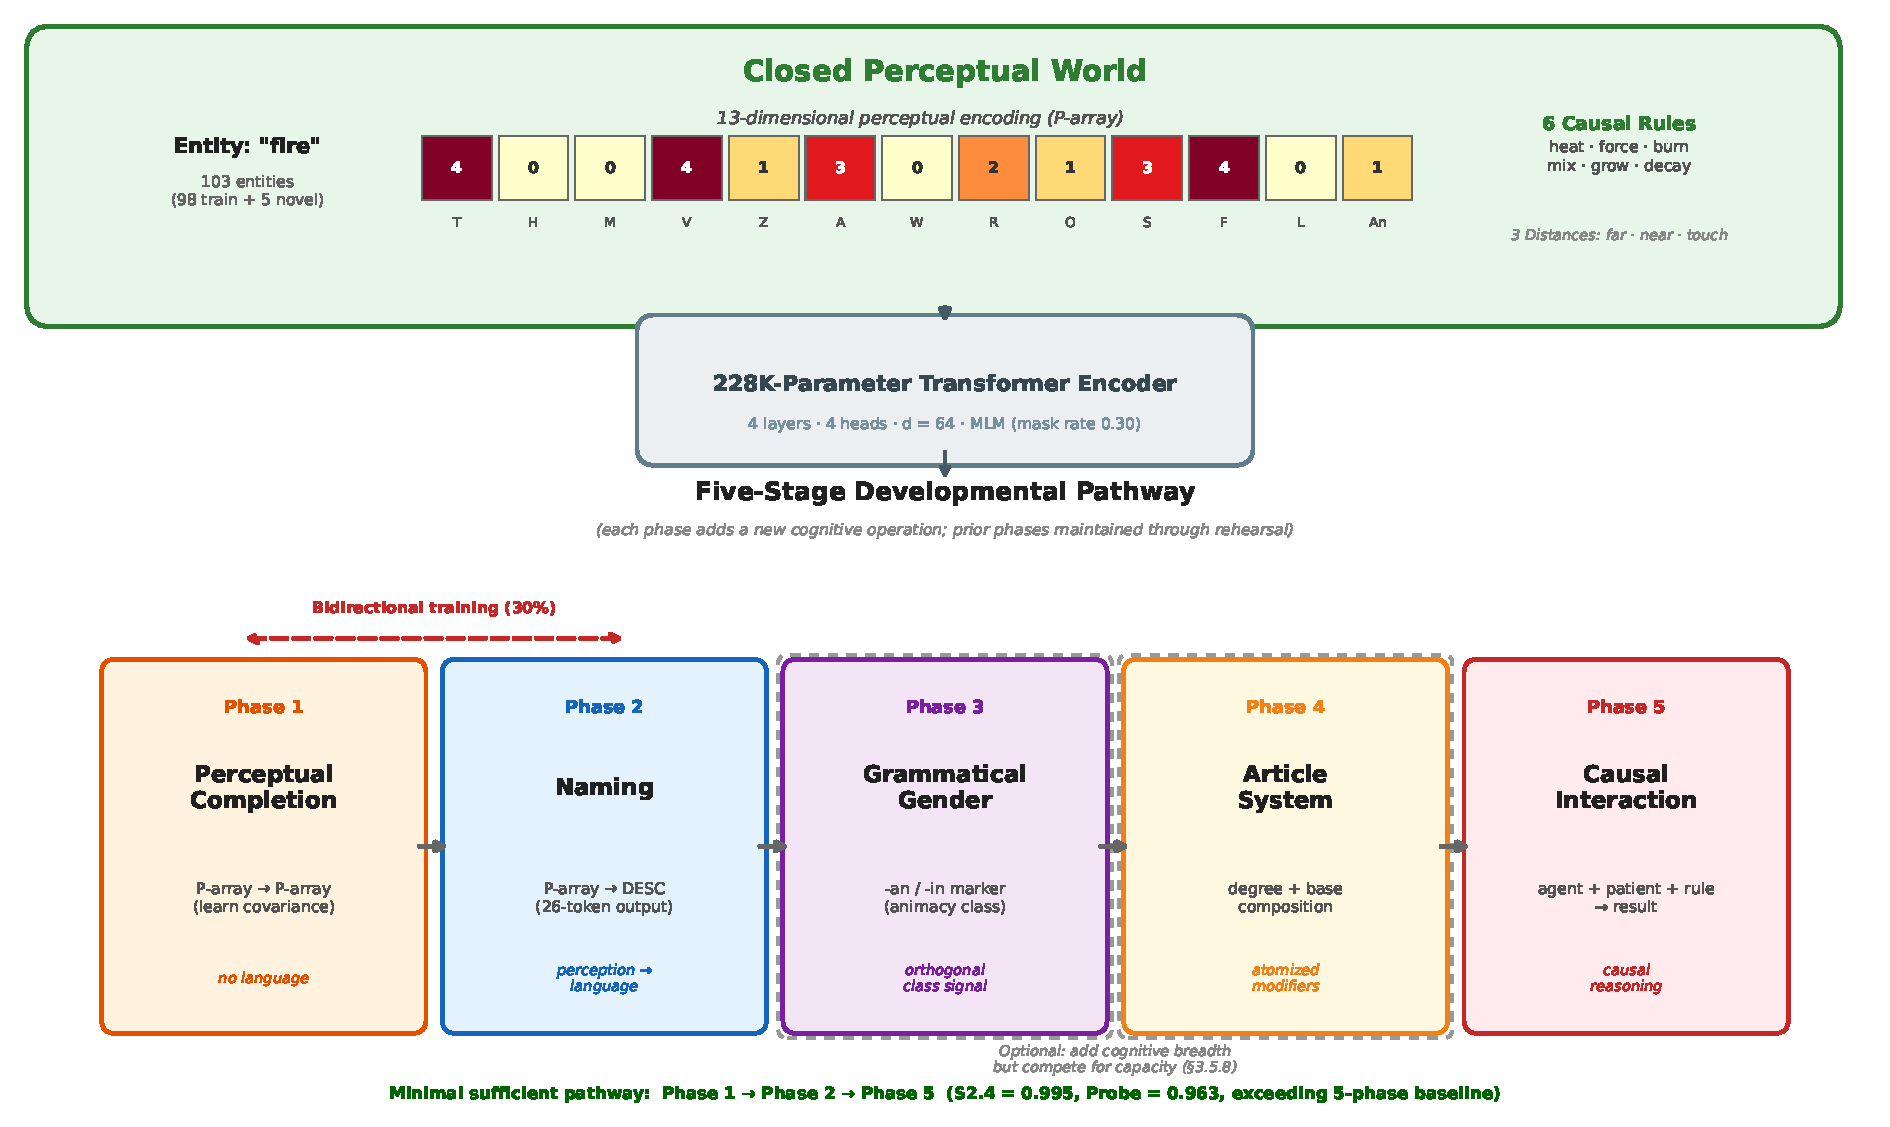
\includegraphics[width=\textwidth]{figures/Fig1_System_Architecture.pdf}
\caption{\textbf{System Architecture.} The closed perceptual world contains 103 entities, each defined by a 13-dimensional sensory encoding. The model receives perceptual input (P-array) and produces linguistic output (DESC tokens) through a developmental pathway. Six causal rules govern entity interactions.}
\label{fig:architecture}
\end{figure}

\subsubsection{Distance Attenuation}

Each entity's encoding is defined at touch distance. The system models three observation distances---\textit{far}, \textit{near}, \textit{touch}---with sensory attenuation: visual channels (V, Z, S) and judgment dimensions (L, An) are preserved at all distances; propagation channels (A, F) decay gradually (near: $-1$, far: $-2$, minimum 0); contact channels (T, H, M, R, W, O) are available only at touch and default to the neutral value (2) at other distances. This triples the training data while encoding a physically motivated constraint: some perceptual dimensions require proximity.

\subsection{Developmental Pathway}

The model traverses five phases in fixed order, followed by a sixth phase that tests whether language can operate without perceptual input (\S3.8). Each phase introduces a qualitatively new cognitive operation while maintaining prior capabilities through built-in rehearsal. This is not curriculum learning in the standard sense~\cite{bengio2009}, which manipulates difficulty gradients. Here, each phase constructs a different cognitive environment---a new kind of thing the model must do.

\begin{table}[htbp]
\centering
\small
\begin{tabular}{cllc}
\toprule
Phase & Name & New cognitive operation & Max steps \\
\midrule
1 & Perceptual completion & Learn covariance structure (no language) & 5,000 \\
2 & Naming & Map 13-dim P-array to 26-token description & 5,000 \\
3 & Grammatical gender & Integrate categorical marker (-an/-in) & 5,000 \\
4 & Article system & Learn compositional degree-marker structure & 5,000 \\
5 & Causal interaction & Predict dimension-level consequences & 10,000 \\
6 & Linguistic autonomy & Infer without perceptual input & 5,000 \\
\bottomrule
\end{tabular}
\caption{Developmental pathway. Each phase introduces a new cognitive operation.}
\label{tab:phases}
\end{table}

Each phase includes rehearsal: prior-phase sequences are mixed into training batches at empirically calibrated proportions. In Phase 5, interaction sequences are repeated 10$\times$ while naming sequences appear 1$\times$ each and perceptual sequences 3$\times$, ensuring that new material dominates while prior capabilities are maintained at $>$95\% accuracy. Early stopping triggers when loss $<$ 0.25 and accuracy $\geq$ 0.95.

\subsection{Model Architecture}

The model is a standard Transformer encoder~\cite{vaswani2017} with 4 layers, 4 attention heads per layer, embedding dimension $d = 64$, feedforward dimension 256, pre-norm (LayerNorm before attention and feedforward), and dropout 0.1, totaling $\sim$228,000 parameters. Maximum sequence length: 48 tokens. Training objective: masked language modeling (MLM), mask rate 0.30. Optimizer: AdamW (lr = $3 \times 10^{-4}$, weight decay = 0.01).

The architecture is deliberately minimal---no post-2017 innovations. The goal is not benchmark performance; it is a system small enough that every mechanism can be inspected, yet capable of grounded generalization and causal reasoning.

Cross-parameter validation: scaling from $d = 32$ (63K parameters) to $d = 256$ (3.3M parameters) produces the same qualitative result pattern across a 50-fold parameter range, confirming that observed capacities reflect training design, not model capacity (\S3.1.5).

\subsection{Bidirectional Training}

In the default (unidirectional) configuration, P-array tokens are context and DESC tokens are masked. In the bidirectional configuration, each S2-format batch has a fixed probability (reverse ratio) of masking P-array tokens instead. We test 0\% (unidirectional), 15\%, and 30\% (bidir30, the primary experimental model). This design directly tests whether symbol grounding is automatically bidirectional or requires explicit reverse training.

%==============================================================================
\section{Results}
%==============================================================================

\subsection{Forward Pathway: Perception Generates Language}

\subsubsection{Convergence Across Developmental Phases}

The developmental pathway converges reliably across all phases (Table~\ref{tab:forward}). Perceptual reconstruction (S1) and the later interaction and autoregressive phases (S2.4--S2.5) exceed 92\%, while the naming and gender description phases stabilize near 80\%, reflecting the greater combinatorial complexity of mapping 13 perceptual dimensions to discrete linguistic tokens. Across five random seeds (42, 123, 456, 789, 1024), the forward pathway shows minimal variance: S1 perceptual reconstruction $= 0.925 \pm 0.002$, S2.4 interaction $= 0.961 \pm 0.008$, S2.5 autoregressive $= 0.983 \pm 0.010$.

\begin{table}[htbp]
\centering
\small
\begin{tabular}{lccc}
\toprule
Metric & Mean $\pm$ Std & Min & Max \\
\midrule
S1 Perceptual reconstruction & $0.925 \pm 0.002$ & 0.923 & 0.927 \\
S2.1 Naming & $0.802 \pm 0.040$ & 0.741 & 0.864 \\
S2.2 Gender description & $0.811 \pm 0.038$ & 0.740 & 0.854 \\
S2.4 Interaction & $0.961 \pm 0.008$ & 0.953 & 0.975 \\
S2.5 Autoregressive & $0.983 \pm 0.010$ & 0.964 & 0.990 \\
Held-out probes & $0.814 \pm 0.018$ & 0.795 & 0.846 \\
\bottomrule
\end{tabular}
\caption{Forward pathway convergence (5 seeds, bidir30 model).}
\label{tab:forward}
\end{table}

\subsubsection{Phase Transition: From Perception to Language}

At the onset of Phase 2, the model's dominant output at DESC positions consists of perceptual-level tokens; it attempts to describe entities using the representational vocabulary of Phase 1. Across five seeds, the P-token ratio averages $0.65 \pm 0.19$ at step 500, while correct DESC-token accuracy averages $0.14 \pm 0.09$. The two curves cross at approximately step 850. Beyond the crossover, perceptual-level outputs decline monotonically toward zero while linguistic accuracy accelerates toward convergence. All five seeds converge between steps 1,394 and 1,598 (accuracy $>$ 0.95).

The transition is abrupt, not gradual. Before the crossover, the model predominantly produces tokens from the wrong vocabulary. After the crossover, linguistic tokens dominate and rapidly consolidate. This phase transition makes the developmental pathway's core claim visible: perception generates language through a representational shift.

\begin{figure}[htbp]
\centering
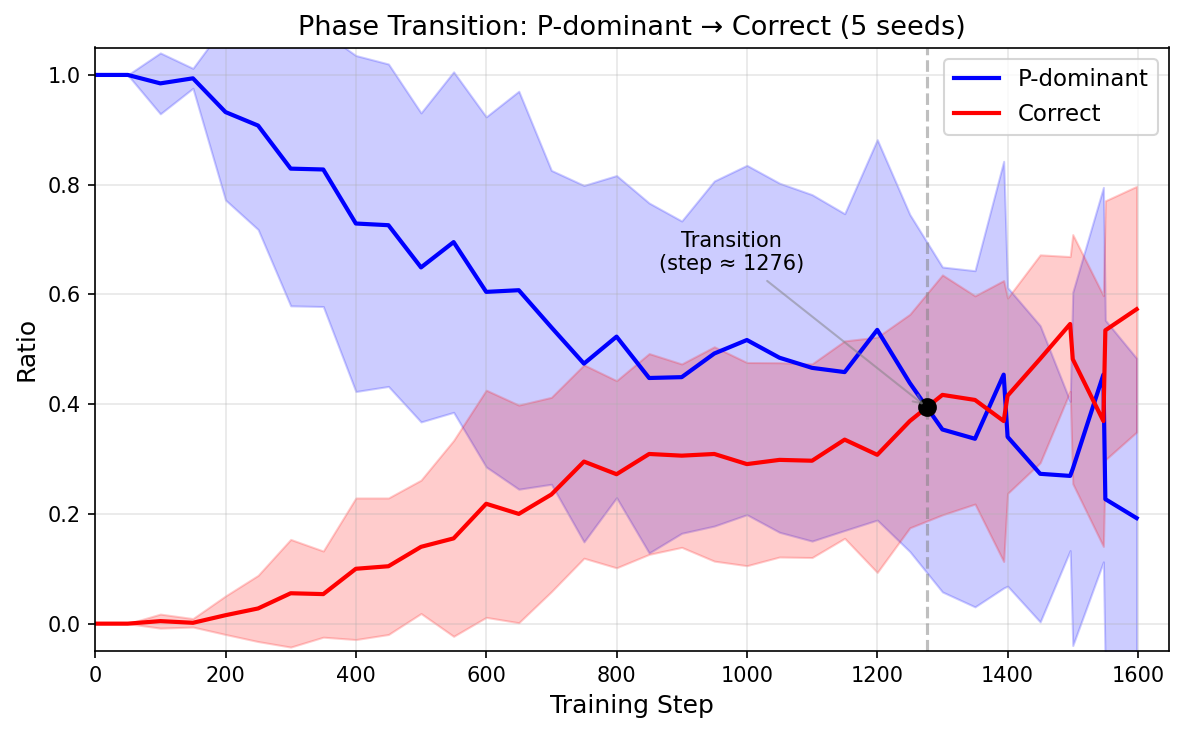
\includegraphics[width=0.9\textwidth]{figures/phase_transition.png}
\caption{\textbf{Phase Transition from Perception to Language.} At Phase 2 onset, the model's dominant output at DESC positions consists of perceptual-level tokens (P-token ratio $\approx 0.65$). The curves cross at approximately step 850. Beyond the crossover, linguistic accuracy accelerates toward convergence while P-token ratio declines to zero. All five seeds converge between steps 1,394--1,598.}
\label{fig:phase_transition}
\end{figure}

\subsubsection{Generalization to Novel Entities}

Five entities withheld entirely from training are tested at evaluation time. Across five seeds, the bidir30 model correctly predicts $7.0 \pm 1.3$ out of 13 perceptual dimensions per novel entity (chance = 2.6/13). When bidirectional training is removed (reverse ratio = 0\%), novel entity generalization drops to $3.0 \pm 1.3$, near chance. The contrast is direct: without explicit reverse training, the model fails to extract per-dimension rules that transfer to unseen entities.

\subsubsection{Rule-Based Composition, Not Memorization}

The decisive test comes from the reverse pathway (\S3.3.3), where the C-group disambiguation experiment directly pits rule-based inference against name-based retrieval. Across five seeds, the model follows per-dimension rules from the linguistic description rather than retrieving stored encodings by name, at a ratio of 5.0:1. The model applies these mapping rules compositionally, without recalling stored entities.

\subsubsection{Scaling Analysis: Training Design, Not Model Capacity}

To test whether the developmental pathway's success depends on model capacity, we train four architectures with identical structure (4 layers, 4 attention heads) under identical bidir30 training, varying only the embedding dimension $d$:

\begin{table}[htbp]
\centering
\small
\begin{tabular}{lccccc}
\toprule
Model & $d$ & Parameters & S2.4 & Probe & Novel (/13) \\
\midrule
XS & 32 & 63K & 0.980 & 0.889 & 8.2 \\
S (5 seeds) & 64 & 228K & $0.961 \pm 0.008$ & $0.814 \pm 0.018$ & $7.0 \pm 1.3$ \\
M & 128 & 841K & 0.973 & 0.889 & 9.2 \\
L & 256 & 3.3M & 0.933 & 0.846 & 9.0 \\
\bottomrule
\end{tabular}
\caption{Scaling analysis (all 4-layer, 4-head, bidir30).}
\label{tab:scaling}
\end{table}

Across a 50-fold range in parameter count, all three core metrics remain flat. No metric shows monotonic improvement with scale; the largest model (L, 3.3M parameters) performs slightly below the smallest (XS, 63K) on interaction accuracy. The implication is direct: given the developmental training design, a 63K-parameter model acquires the same qualitative capabilities as one 50 times its size. The bottleneck is the structure of the training environment, not representational capacity.

\subsection{Causal Reasoning: From Naming to Understanding}

\subsubsection{Interaction Prediction}

When two entities interact under one of six causal rules, the model predicts the dimension-level consequences for the patient entity. On held-out entity pairs (combinations never seen during training), overall accuracy is $0.814 \pm 0.018$ across five seeds (Table~\ref{tab:forward}). The variance across seeds is small (std = 0.018), confirming that causal reasoning ability is a stable product of the developmental pathway.

\subsubsection{Animacy Functionalization}

Entities with An=0 (inanimate) never appear as agents during training; they are always patients. At test time, we place An=0 entities in the agent role. The model correctly applies the causal rules regardless of animacy status, generalizing to a configuration never encountered during training.

This result transforms animacy from a classification label into a functional category. The model has learned what animacy \emph{is} (a perceptual dimension), not merely what animacy \emph{correlates with} (being an agent). The gender-marking system contributes to this functional understanding: removing both gender markers from interaction sequences reduces accuracy from $0.960 \pm 0.008$ to $0.773 \pm 0.160$ across five seeds (\S3.4.3). Gender swap experiments further reveal that the markers causally control predictions on three animacy-related dimensions---vitality (L), olfactory noxiousness (F), and animacy (An)---while leaving the remaining ten dimensions unaffected.

The forward pathway, from perception through language to causal reasoning, is complete. The model has moved from naming to understanding. Before asking whether this pathway is bidirectional (\S3.3), we examine the representational architecture that makes it possible: the separation of perception, object identity, and language into three independently operable layers.

\subsubsection{Representational Architecture: Three-Layer Separation}

The system's design enforces a three-layer representational structure---perception, object identity, and language---that are independently operable yet connected by learned mappings. This separation is the architectural foundation that enables variable isolation, compositional generalization, and the full ablation framework reported in \S3.4--3.7.

\paragraph{Layer 1: Pure Perception (P-array).} In Phase 1, the model operates exclusively on perceptual encodings: 13-dimensional arrays with no linguistic tokens, no entity names, no class markers. The model learns the covariance structure of the perceptual space (which dimensions predict which) before it has any words. This layer is where the model discovers that bright entities tend to be dry, heavy entities tend to be loud, and living entities tend to be pungent---regularities that \S3.6.1 will show persist into the fully trained model as emergent dimensional covariance.

\paragraph{Layer 2: Object Identity (Name + Gender).} Entity names and gender markers constitute an identity layer orthogonal to perceptual content. The independence of this layer from Layer 1 is directly measured: masking the entity name produces no accuracy change on perceptual-to-linguistic mapping (\S3.4.1, $\Delta = 0.000$), and linear probing at name positions yields chance-level accuracy for dimensional information across all layers (\S3.7.2, 0.29--0.33). The model does not route perceptual information through entity identity. Conversely, gender markers selectively modulate exactly three biology-related dimensions (\S3.4.2) without affecting the other ten, demonstrating that class-based identity provides an independent information channel that interacts with, but does not substitute for, perceptual content.

\paragraph{Layer 3: Language (Degree Marker + Base Word).} The 26-token linguistic description (13 degree-marker + base-word pairs) constitutes a compositional encoding in which each perceptual dimension is independently named and graded. This layer is the output target during forward training and the input during reverse training (\S3.3). Its compositional structure---each pair encodes exactly one dimension at exactly one level---is what enables per-dimension ablation (\S3.6), per-dimension accuracy measurement, and the disambiguation experiment (\S3.3.3) that pits rule-based inference against name-based retrieval.

\paragraph{The Separations Are Measured, Not Assumed.} Three experimental results confirm that these layers are operationally independent. Phase 1 perceptual reconstruction (S1 = 0.925) demonstrates that the model extracts structured perceptual knowledge before any linguistic token is introduced. Name removal has zero effect on forward accuracy (\S3.4.1), confirming that the model maps perception to language through per-dimension rules rather than entity lookup. And gender swap changes predictions on exactly three dimensions while leaving ten untouched (\S3.4.2); removing both gender markers collapses interaction accuracy by 18.7\% (\S3.4.3). The markers carry information that neither the perceptual encoding nor the linguistic description alone provides.

In a standard LLM, ``fire'' is a single token whose representation is shaped entirely by distributional co-occurrence with other tokens; perception, identity, and language are collapsed into a single embedding. In our system, the perceptual representation of fire (T=4, H=0, M=0, V=4, ...) exists independently of its name (``fire'') and independently of its linguistic description (``max therm, nul dur, ...''). Each layer can be independently manipulated, and the mappings between layers can be independently measured. This is the architectural condition that makes the diagnostic framework of \S3.4--3.7 possible.

\S3.3 now asks whether the perception-to-language bridge established in \S3.1--3.2 is automatically bidirectional, or whether the reverse direction must be separately earned.

\subsection{Bidirectional Bridging: Language Reconstructs Perception}

\subsubsection{Unidirectional Training Produces Near-Zero Reverse Capability}

When the model is trained only in the perception-to-language direction (reverse-ratio = 0\%), reverse inference accuracy is near-chance: $0.079 \pm 0.041$ for trained entities. Symbol grounding is not automatically bidirectional. The forward bridge does not leak backward.

\subsubsection{Bidirectional Training Enables Reverse Inference}

At reverse-ratio = 30\% (bidir30), reverse accuracy rises from zero to substantial levels across five seeds:

\begin{table}[htbp]
\centering
\small
\begin{tabular}{lccc}
\toprule
Test Group & Mean $\pm$ Std & Min & Max \\
\midrule
A $\cdot$ Trained entities & $0.654 \pm 0.115$ & 0.432 & 0.761 \\
B $\cdot$ Novel entities & $0.612 \pm 0.112$ & 0.415 & 0.739 \\
C $\cdot$ Name-description mismatch & $0.654 \pm 0.124$ & 0.415 & 0.769 \\
D $\cdot$ Fictitious encodings & $0.492 \pm 0.124$ & 0.308 & 0.692 \\
E $\cdot$ Interaction results & $0.843 \pm 0.106$ & 0.656 & 0.969 \\
F $\cdot$ Held-out interaction pairs & $0.791 \pm 0.096$ & 0.658 & 0.940 \\
\bottomrule
\end{tabular}
\caption{Reverse inference accuracy (5 seeds, bidir30).}
\label{tab:reverse}
\end{table}

\subsubsection{Disambiguation: Rules, Not Memory}

The C group is the decisive test. Each sequence pairs one entity's name with a different entity's complete encoding. If the model predicts the P-array matching the \emph{description}, it is using per-dimension rules. If it predicts the P-array matching the \emph{name}, it is retrieving from memory.

\begin{table}[htbp]
\centering
\small
\begin{tabular}{lcccc}
\toprule
Seed & Desc-match & Name-match & Neither & Ratio \\
\midrule
1024 & 58 & 6 & 35 & 9.7:1 \\
123 & 64 & 9 & 21 & 7.1:1 \\
42 & 37 & 15 & 61 & 2.5:1 \\
456 & 58 & 10 & 26 & 5.8:1 \\
789 & 55 & 14 & 28 & 3.9:1 \\
\textbf{Mean $\pm$ Std} & \textbf{54.4 $\pm$ 9.2} & \textbf{10.8 $\pm$ 3.3} & \textbf{34.2 $\pm$ 15.0} & \textbf{5.0:1} \\
\bottomrule
\end{tabular}
\caption{C-group disambiguation (5 seeds). The model follows rules, not names.}
\label{tab:cgroup}
\end{table}

All five independently trained models choose the description over the name. The model performs reverse inference by applying per-dimension rules from the linguistic description, not by looking up a stored encoding associated with the entity name.

\begin{figure}[htbp]
\centering
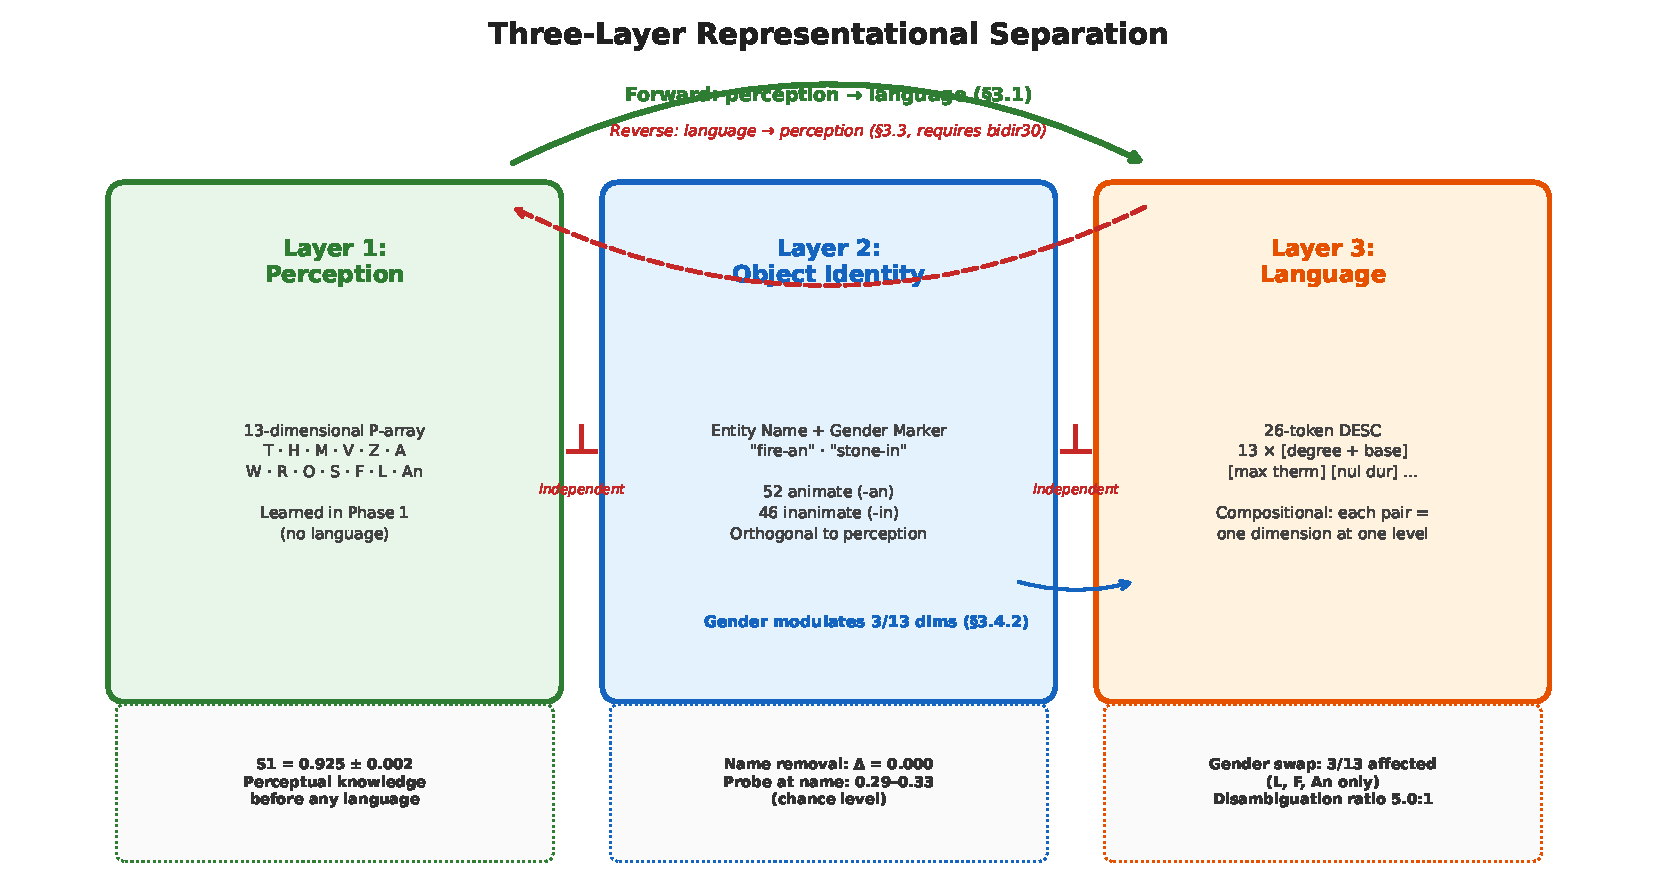
\includegraphics[width=0.95\textwidth]{figures/Fig3_Three_Layer_Separation.pdf}
\caption{\textbf{Three-Layer Separation in Bidirectional Bridging.} The model separates forward inference (perception $\rightarrow$ language), reverse inference (language $\rightarrow$ perception), and disambiguation (rule-based vs.\ memory-based retrieval). The C-group test directly pits per-dimension rules against name-based retrieval; across five seeds, the model follows descriptions over names at a 5.0:1 ratio.}
\label{fig:three_layer}
\end{figure}

\subsubsection{Resource Competition: Context Richness Determines Efficiency}

Three reverse-ratio configurations (0\%, 15\%, 30\%) reveal an asymmetry:

\begin{table}[htbp]
\centering
\small
\begin{tabular}{lccc}
\toprule
Metric & 0\% (n=5) & 15\% (n=5) & 30\% (n=5) \\
\midrule
A reverse (name) & $0.079 \pm 0.041$ & $0.540 \pm 0.032$ & $0.607 \pm 0.068$ \\
B reverse (novel) & $0.089 \pm 0.030$ & $0.501 \pm 0.021$ & $0.575 \pm 0.073$ \\
C reverse (mismatch) & $0.092 \pm 0.057$ & $0.545 \pm 0.032$ & $0.605 \pm 0.081$ \\
D reverse (fictional) & $0.055 \pm 0.026$ & $0.425 \pm 0.020$ & $0.447 \pm 0.047$ \\
E reverse (interact) & $0.013 \pm 0.008$ & $0.469 \pm 0.030$ & $0.809 \pm 0.084$ \\
F reverse (probes) & $0.010 \pm 0.008$ & $0.393 \pm 0.023$ & $0.764 \pm 0.088$ \\
A forward (name) & $0.646 \pm 0.098$ & $0.597 \pm 0.131$ & $0.519 \pm 0.049$ \\
E forward (interact) & $0.908 \pm 0.011$ & $0.923 \pm 0.009$ & $0.893 \pm 0.024$ \\
\bottomrule
\end{tabular}
\caption{Resource competition across reverse ratios (5 seeds each).}
\label{tab:resource}
\end{table}

The table reveals two distinct regimes. In the name format (sparse context: only entity name, P-array, and description), forward and reverse directions compete: A forward drops from 0.646 to 0.519 as reverse ratio increases from 0\% to 30\%, while A reverse rises from 0.079 to 0.607. In the interaction format (rich context: two entities, gender markers, case, and rule), no such trade-off appears: E forward remains stable (0.908 $\rightarrow$ 0.893), while E reverse rises sharply from near-chance (0.013) to 0.809. Richer context transforms bidirectional training from zero-sum competition into mutual benefit.

This resource competition also explains the gap between the 0\% and bidir30 models on novel entity generalization in the forward pathway (\S3.1.3): the 0\% model achieves only $3.0 \pm 1.3$ novel dimensions (near chance) while the bidir30 model averages $7.0 \pm 1.3$/13. Rather than degrading generalization, bidirectional pressure forces the model to extract more abstract, per-dimension rules that transfer to unseen entities.

\subsection{Categorical Markers as Independent Reasoning Tools}

\subsubsection{Name Removal Has No Effect; Gender Removal Does}

In single-entity descriptions, masking the entity name produces no accuracy change ($0.809 \pm 0.038$ vs.\ Full = $0.811 \pm 0.038$). Masking the gender marker produces a small but consistent drop ($0.805 \pm 0.040$, $\Delta = -0.6\%$). The model maps perception to language through dimension-level rules that do not depend on entity identity.

\subsubsection{Gender Swap Causally Controls Three Dimensions}

Swapping gender markers (-an $\leftrightarrow$ -in) while keeping all perceptual information constant reveals which dimensions are causally influenced by class membership:

\begin{table}[htbp]
\centering
\small
\begin{tabular}{lccc}
\toprule
Dimension & Full (mean $\pm$ std) & Swap (mean $\pm$ std) & $\Delta$ (mean $\pm$ std) \\
\midrule
L (vitality) & $0.899 \pm 0.065$ & $0.812 \pm 0.106$ & $-0.087 \pm 0.066$ \\
F (olfactory) & $0.875 \pm 0.069$ & $0.814 \pm 0.068$ & $-0.061 \pm 0.042$ \\
An (animacy) & $0.951 \pm 0.036$ & $0.802 \pm 0.187$ & $-0.149 \pm 0.153$ \\
All other dims (10) & --- & --- & $|\Delta| < 0.015$ \\
\bottomrule
\end{tabular}
\caption{Gender swap per-dimension effect (5 seeds). Three biology-related dimensions respond.}
\label{tab:genderswap}
\end{table}

Three dimensions respond to the gender marker: vitality, olfactory noxiousness, and animacy. The remaining ten are unaffected. All three affected dimensions relate to biological status (aliveness, organic chemistry, agency), suggesting the model treats them as a coherent cluster.

\subsubsection{Interaction Format: Redundancy and Collapse}

In interaction sequences, each entity carries its own gender marker, providing two class-based signals per sequence.

\begin{table}[htbp]
\centering
\small
\begin{tabular}{lc}
\toprule
Condition & Mean $\pm$ Std \\
\midrule
Full (both markers) & $0.960 \pm 0.008$ \\
No agent marker & $0.928 \pm 0.029$ \\
No patient marker & $0.949 \pm 0.014$ \\
No both markers & $0.773 \pm 0.160$ \\
\bottomrule
\end{tabular}
\caption{Gender ablation in interaction format (5 seeds).}
\label{tab:genderablation}
\end{table}

Removing one marker produces modest degradation; the remaining marker compensates. Removing both causes a collapse ($\Delta = -18.7\%$). The two gender markers form a redundant system.

\subsection{Developmental Order Is Causally Necessary}

\subsubsection{Phase Ablation}

To test whether the developmental pathway is causally necessary or merely a convenient training schedule, we train ablation models with individual phases removed or with all phases shuffled. All conditions use reverse-ratio = 0.3 and max\_phase = 5, validated with at least three random seeds.

\begin{table}[htbp]
\centering
\small
\begin{tabular}{lcccccc}
\toprule
Model & S1 & S2.1 & S2.2 & S2.4 & S2.5 & Probe \\
\midrule
Baseline (5 seeds) & 0.925 & 0.802 & 0.811 & 0.961 & 0.983 & 0.814 \\
$\Delta$Ph1 (skip perception) & 0.878 & 0.723 & 0.813 & 0.960 & 0.984 & 0.829 \\
$\Delta$Ph2 (skip naming) & 0.894 & 0.838 & 0.781 & 0.981 & 0.983 & 0.926 \\
$\Delta$Ph3 (skip gender) & 0.925 & 0.788 & 0.531 & 0.970 & 0.976 & 0.860 \\
$\Delta$Ph4 (skip articles) & 0.923 & 0.712 & 0.649 & 0.990 & 0.992 & 0.929 \\
$\Delta$Ph5 (skip interaction) & 0.933 & 0.789 & 0.938 & \textbf{0.001} & 0.000 & 0.003 \\
Shuffle (3 seeds) & 0.927 & 0.855 & 0.966 & 0.427 & 0.366 & 0.308 \\
\bottomrule
\end{tabular}
\caption{Phase ablation results. $\Delta$Ph5 eliminates causal reasoning entirely.}
\label{tab:ablation}
\end{table}

\subsubsection{Removing Interaction Phase: Deterministic Failure}

$\Delta$Ph5 (training phases [1,2,3,4], skipping causal interaction) produces S2.4 $= 0.001 \pm 0.000$ across three seeds. No seed achieves above-chance interaction accuracy. The standard deviation is zero: the result is deterministic rather than probabilistic. Causal reasoning does not partially degrade; it is absent.

\subsubsection{Shuffled Order: Same Data, Collapsed Capacity}

The Shuffle model receives identical training data in scrambled order [5,4,1,3,2]. Results:
\begin{itemize}
    \item S2.4 interaction: $0.427 \pm 0.308$ (vs.\ Baseline $0.961 \pm 0.008$)
    \item S2.5 autoregressive: $0.366 \pm 0.250$
    \item Probes (held-out): $0.308 \pm 0.193$
\end{itemize}

The mean drops by more than half, but the variance tells the deeper story. Baseline S2.4 standard deviation is 0.008; Shuffle standard deviation is 0.308, a 38-fold increase. Under the correct developmental sequence, the outcome is predictable across random initializations. Under shuffled order, whether the model learns depends on the accident of initialization.

\subsubsection{Low-Order Capacities Are Order-Immune}

Shuffle achieves S2.1 $= 0.855 \pm 0.091$ and S2.2 $= 0.966 \pm 0.020$, both at or above Baseline. Naming and description survive or improve under scrambled order. Only higher-order capacities (interaction, causal reasoning, generalization to held-out pairs) collapse.

This dissociation is the key feature of the result. Developmental order does not act as a global quality control that makes everything better or worse; it selectively governs whether higher-order capacities emerge. Simple perceptual-to-linguistic mappings can be learned regardless of when the data arrives, but causal reasoning requires that those mappings already be in place.

\subsubsection{Non-Uniform Phase Contributions}

An unexpected finding emerges from the $\Delta$Ph4 ablation. Skipping the article phase produces Probe $= 0.929 \pm 0.021$, higher than the Baseline value of $0.814 \pm 0.018$. Removing article training frees model capacity that is reallocated to interaction learning. The developmental phases do not all contribute positively to every downstream capability; some compete for the same representational resources.

\subsubsection{Extended Permutation Analysis}

Four additional permutations, each validated across three seeds, test specific hypotheses about which ordering constraints are necessary:

\begin{table}[htbp]
\centering
\small
\begin{tabular}{lccccccc}
\toprule
Model & S1 & S2.1 & S2.2 & S2.4 & S2.5 & Probe & Order \\
\midrule
S-A (swap 4$\leftrightarrow$5) & 0.926 & 0.808 & 0.921 & 0.835 & 0.943 & 0.595 & [1,2,3,5,4] \\
S-B (gender first) & 0.928 & 0.816 & 0.735 & 0.982 & 0.983 & 0.932 & [3,1,2,4,5] \\
S-C (interaction first) & 0.935 & 0.999 & 0.961 & \textbf{0.016} & 0.040 & 0.020 & [5,2,4,1,3] \\
$\Delta$34 (skip Ph3+Ph4) & 0.923 & 0.606 & 0.299 & \textbf{0.995} & 0.996 & \textbf{0.963} & [1,2,5] \\
\bottomrule
\end{tabular}
\caption{Extended permutation results (3 seeds each). S-C shows interaction-first collapse. $\Delta$34 shows minimal pathway superiority.}
\label{tab:extended}
\end{table}

\subsubsection{Interaction-First Collapse Is Robust}

The S-C permutation [5,2,4,1,3] produces S2.4 $= 0.016 \pm 0.018$, replicating the original Shuffle result with even more severe collapse. Two different interaction-first orderings both eliminate causal reasoning. Meanwhile, low-order capacities reach ceiling: S2.1 = 0.999, S2.2 = 0.961. The collapse is not an artifact of one particular scramble. Presenting causal interaction data before the model has built any perceptual or linguistic foundation produces the same failure regardless of how the remaining phases are arranged.

\subsubsection{The Minimal Sufficient Pathway}

The $\Delta$34 result is the most consequential finding in the extended analysis. A model trained on only three phases---perception (Phase 1), naming (Phase 2), and interaction (Phase 5)---achieves S2.4 $= 0.995 \pm 0.003$ and Probe $= 0.963 \pm 0.022$. Both metrics \emph{exceed} the five-phase Baseline (S2.4 = 0.961, Probe = 0.814) by a substantial margin.

This extends the $\Delta$Ph4 finding (\S3.5.5) to its logical conclusion. Phase 3 (gender) and Phase 4 (degree markers) are not prerequisites for causal reasoning. When freed from learning gender classification and compositional degree-marker encoding, the 228K-parameter model allocates its full capacity to the perception--naming--interaction pathway, and the result is near-ceiling performance on both causal reasoning and held-out generalization.

The cost appears in the capabilities the skipped phases were designed to support. S2.2 (gender description) drops to 0.299, since the model has never encountered gender training data. S2.1 (naming) drops to 0.606, since degree markers are absent and the naming format becomes harder to learn. The intermediate phases add genuine cognitive capabilities (class-based reasoning, compositional description), but these capabilities compete with causal reasoning for the model's limited representational capacity.

\subsubsection{Revised Claim: What Is and Is Not Causally Necessary}

The extended permutation data supports a three-part decomposition.

\textbf{Perception and naming must precede interaction.} Both interaction-first orderings ([5,4,1,3,2] and [5,2,4,1,3]) collapse S2.4 to near zero; all orderings that place perception and naming before interaction achieve S2.4 $>$ 0.83. Interaction training data is also required: $\Delta$Ph5 yields S2.4 $= 0.001 \pm 0.000$. Together, these establish the causally necessary conditions for causal reasoning.

\textbf{Phase 3 (gender) and Phase 4 (degree markers) are not among these necessary conditions.} The $\Delta$34 model [1,2,5] achieves S2.4 = 0.995 and Probe = 0.963, exceeding the full Baseline on both metrics.

\textbf{Ordering sensitivity exists along a gradient.} Gender can precede perception ([3,1,2,4,5]) without harming causal reasoning (S2.4 = 0.982), though it slightly impairs its own accuracy (S2.2 = 0.735 vs.\ Baseline 0.811). Swapping Phase 4 and 5 ([1,2,3,5,4]) degrades both causal reasoning (S2.4 = 0.835) and generalization (Probe = 0.595), but does not produce the catastrophic collapse seen in interaction-first orderings.

The developmental pathway's core is a three-stage sequence: perceive, name, interact. This sequence is both necessary and sufficient for grounded causal reasoning in this system. The full pathway through Phase 5 adds cognitive breadth (class-based reasoning, compositional description) at a measurable cost to depth (causal reasoning, held-out generalization) in a 228K-parameter model. This capacity trade-off is itself a finding: it establishes that 228K parameters are near the lower bound for the full task, forcing the model to choose between distinct cognitive capabilities.

\subsection{Emergent Dimensional Covariance}

Ablating each of the 13 dimensions (masking its P-token and DESC pair) and measuring the effect on the remaining 12 dimensions produces a 13$\times$13 difference matrix. Selected significant dependencies ($|$effect$| > 0.10$) from the name format:

\begin{table}[htbp]
\centering
\small
\begin{tabular}{lcc}
\toprule
Ablated dimension & Most affected dimension & Effect (mean $\pm$ std) \\
\midrule
V (brightness) & M (moisture) & $+0.299 \pm 0.111$ \\
Z (size) & V (brightness) & $+0.240 \pm 0.124$ \\
A (auditory) & Z (size) & $-0.114 \pm 0.145$ \\
L (vitality) & F (olfactory) & $+0.108 \pm 0.068$ \\
W (weight) & A (auditory) & $+0.108 \pm 0.054$ \\
\bottomrule
\end{tabular}
\caption{Dimension ablation: significant cross-dimensional effects (5 seeds, S2.1 format).}
\label{tab:dimablation}
\end{table}

None of these dependencies were part of the training signal. The model learned them from the statistical structure of the closed world's entity definitions. The L$\rightarrow$F dependency deserves particular attention: ablating vitality increases olfactory prediction accuracy. Two independent methods---one interventional (marker swap) and one observational (dimension ablation)---converge on the same grouping.

\begin{figure}[htbp]
\centering
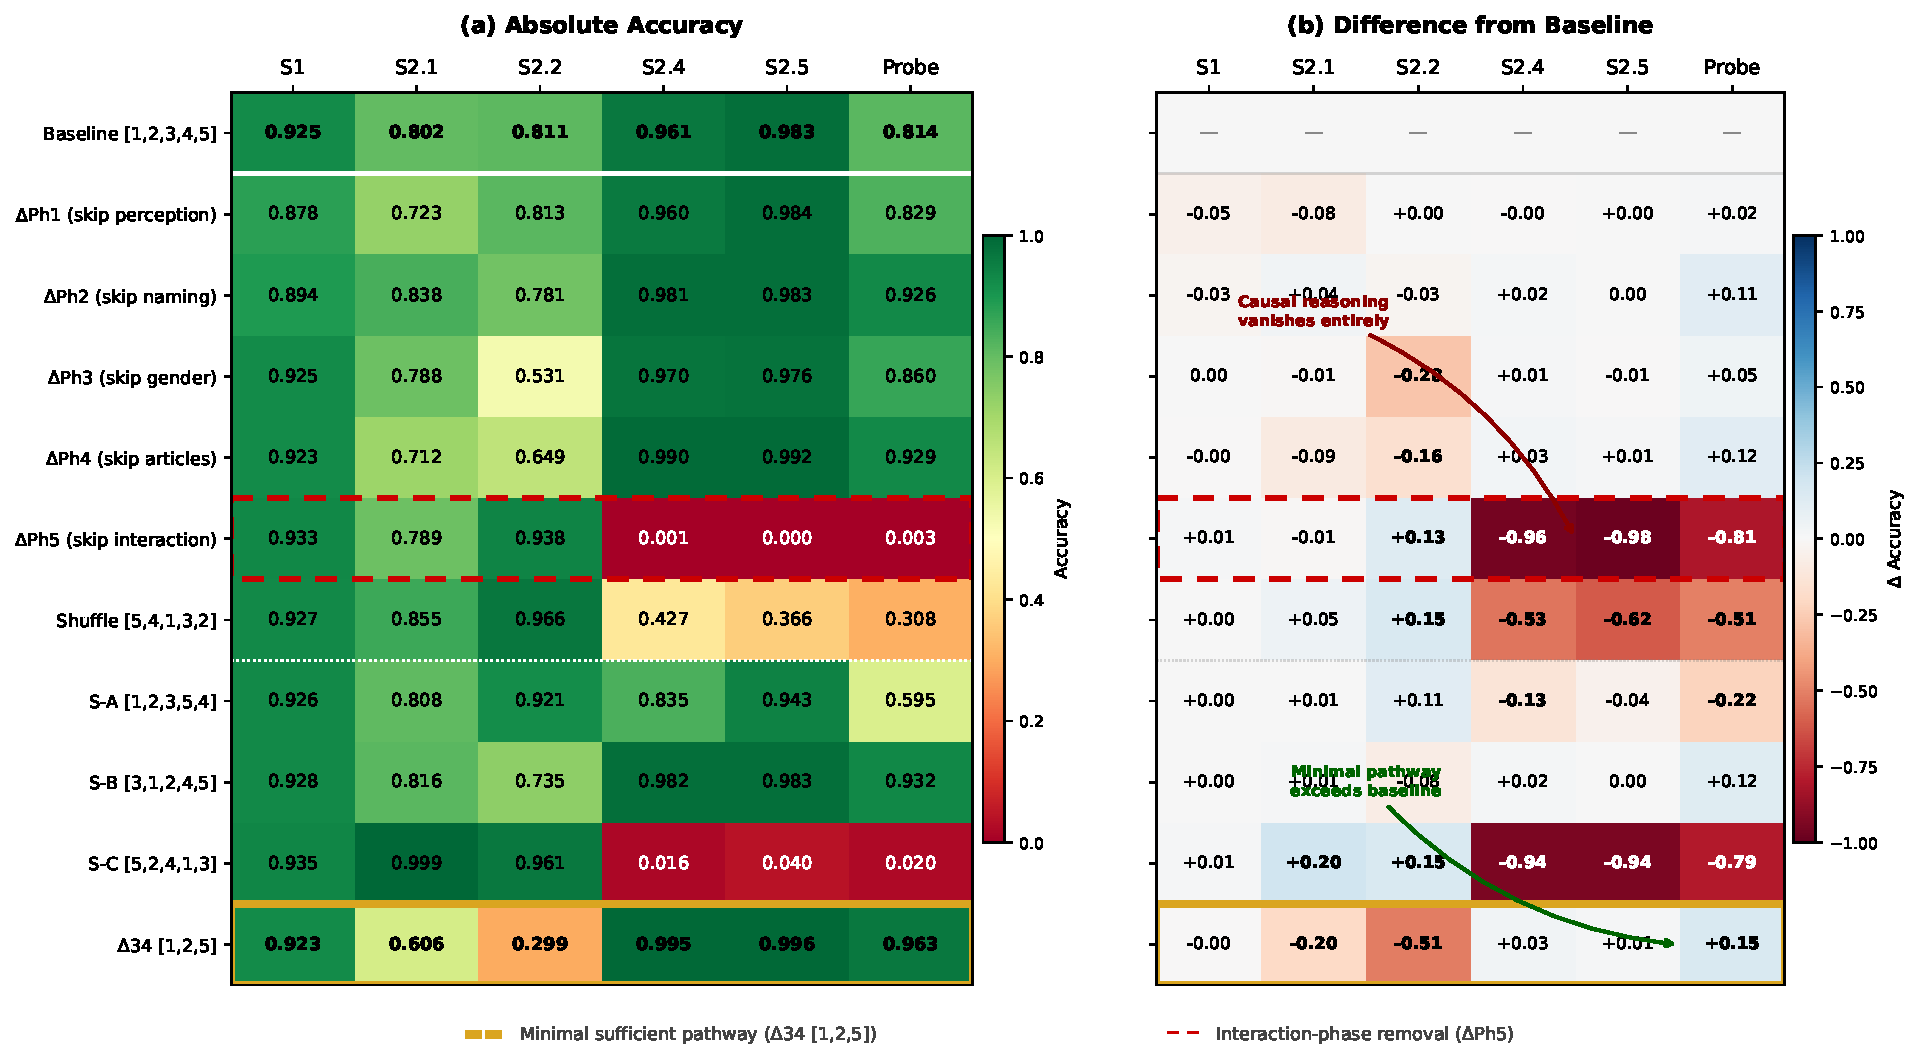
\includegraphics[width=0.85\textwidth]{figures/Fig5_Ablation_Heatmap.pdf}
\caption{\textbf{Phase Ablation Heatmap.} Rows: ablation conditions (Baseline, $\Delta$Ph1--$\Delta$Ph5, Shuffle, and extended permutations S-A, S-B, S-C, $\Delta$34). Columns: evaluation metrics (S1 perceptual, S2.1--S2.5 linguistic, Probe generalization). $\Delta$Ph5 (skip interaction) produces deterministic failure on S2.4 (accuracy = 0.001). Shuffle collapses higher-order capacities while preserving lower-order ones. $\Delta$34 (minimal pathway: perception $\rightarrow$ naming $\rightarrow$ interaction) achieves highest S2.4 and Probe scores.}
\label{fig:ablation_heatmap}
\end{figure}

\subsection{Mechanistic Decomposition}

\subsubsection{Attention Head Specialization}

DESC token predictions attend to their corresponding P-array positions with varying degrees of specificity. Layer 0 is the primary alignment layer across all three seeds tested:

\begin{table}[!ht]
\centering
\small
\begin{tabular}{lc}
\toprule
Head $\cdot$ Dimension & Specificity (mean $\pm$ std) \\
\midrule
L0$\cdot$H0 $\cdot$ T (temperature) & $5.94 \pm 3.42$ \\
L0$\cdot$H1 $\cdot$ H (hardness) & $4.39 \pm 2.68$ \\
L0$\cdot$H0 $\cdot$ W (weight) & $3.91 \pm 0.88$ \\
L0$\cdot$H1 $\cdot$ V (brightness) & $3.63 \pm 2.11$ \\
L1$\cdot$H2 $\cdot$ An (animacy) & $3.52 \pm 1.99$ \\
\bottomrule
\end{tabular}
\caption{Attention specificity by dimension (3 seeds, Layer 0 only).}
\label{tab:attention}
\end{table}

Which head handles which dimension varies across seeds, but the dominance of Layer 0 does not. The dimension-alignment problem is solved in the first layer; subsequent layers handle integration rather than alignment.

\subsubsection{Cross-Dimensional Information Integration}

Linear probing at P-array positions in the final layer reveals how much information each position encodes about dimensions other than its own:

\begin{table}[htbp]
\centering
\small
\begin{tabular}{lc}
\toprule
Metric & Mean $\pm$ Std \\
\midrule
Diagonal (own dimension) & $0.938 \pm 0.007$ \\
Off-diagonal (other dimensions) & $0.608 \pm 0.006$ \\
\bottomrule
\end{tabular}
\caption{Cross-dimensional probing (3 seeds).}
\label{tab:crossdim}
\end{table}

By the output layer, each P-array position encodes substantial information about all 13 dimensions, not just the one it was assigned.

\subsubsection{Information Arrival at Prediction Sites}

Linear probing at masked DESC positions across layers reveals when correct predictions become available:

\begin{table}[htbp]
\centering
\small
\begin{tabular}{lc}
\toprule
Layer & Mean $\pm$ Std \\
\midrule
Layer 0 (embedding) & $0.365 \pm 0.000$ \\
Layer 1 & $0.897 \pm 0.017$ \\
Layer 2 & $0.870 \pm 0.011$ \\
Layer 3 & $0.839 \pm 0.016$ \\
Layer 4 (output) & $0.814 \pm 0.020$ \\
\bottomrule
\end{tabular}
\caption{Masked DESC position probe accuracy by layer (3 seeds).}
\label{tab:infoarrival}
\end{table}

The transition between Layer 0 and Layer 1 is where the work happens: accuracy jumps from 0.365 to 0.897. The model writes the correct answer from the P-array into the masked prediction site during its first computational layer.

\subsubsection{Causal Intervention: Information Flow Direction}

The final analysis replaces the entire P-array's hidden states at each layer with those from a different entity, then measures how much the DESC predictions shift to match the patched entity:

\begin{table}[htbp]
\centering
\small
\begin{tabular}{lc}
\toprule
Patch layer & Mean $\pm$ Std \\
\midrule
Layer 0 & $0.533 \pm 0.048$ \\
Layer 1 & $0.383 \pm 0.075$ \\
Layer 2 & $0.201 \pm 0.048$ \\
Layer 3 & $0.000 \pm 0.000$ \\
\bottomrule
\end{tabular}
\caption{Causal intervention success rate by layer (3 seeds).}
\label{tab:causal}
\end{table}

Information flows from the P-array to DESC positions primarily in Layers 0--1. By Layer 3, patching the P-array produces zero effect; the information has been fully consumed and transferred.

\begin{figure}[htbp]
\centering
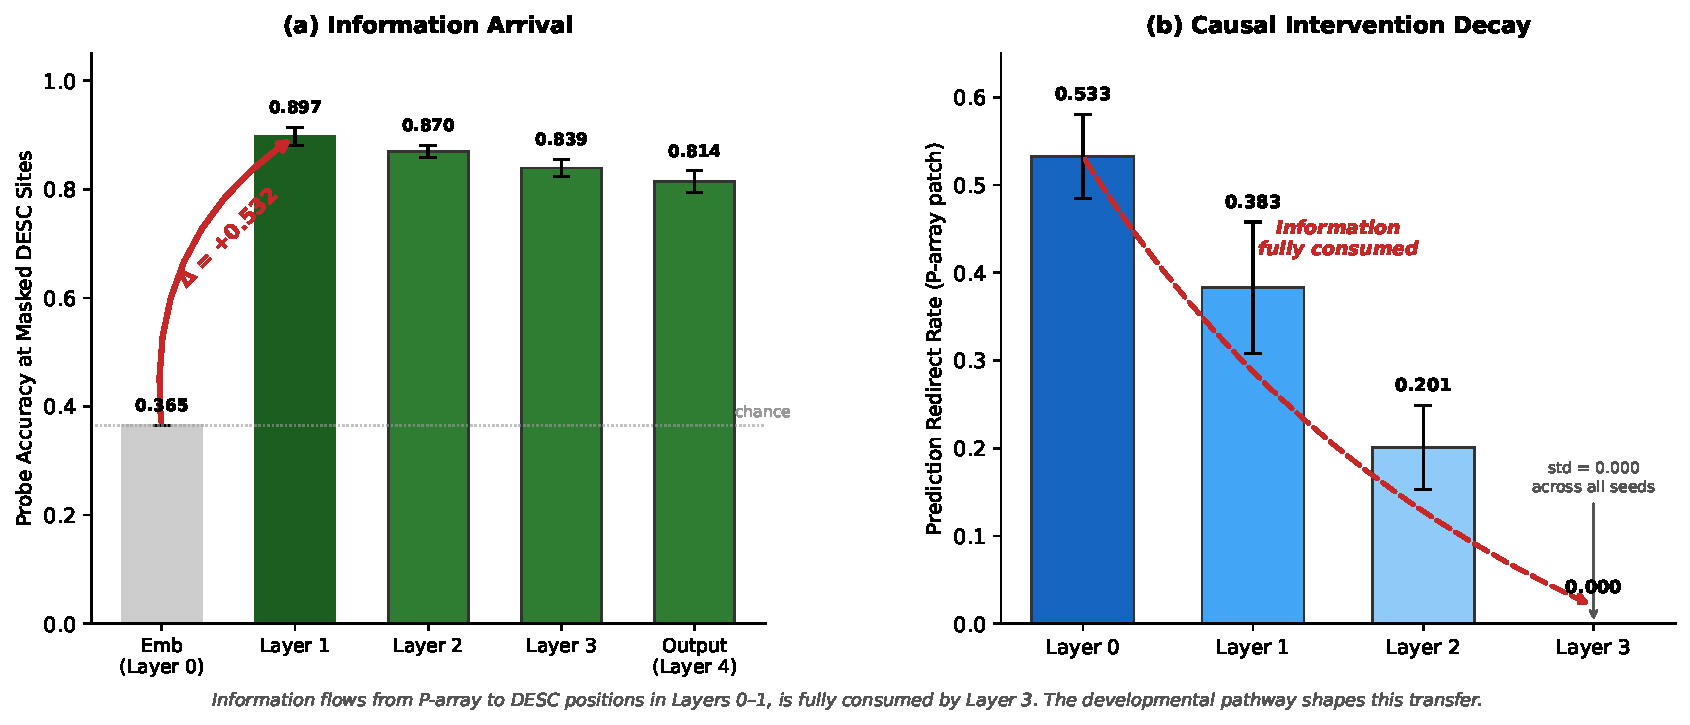
\includegraphics[width=0.95\textwidth]{figures/Fig4_Mechanistic_Decomposition.pdf}
\caption{\textbf{Mechanistic Decomposition.} (a) \textit{Information Arrival}: Linear probing at masked DESC positions shows correct predictions arrive between Layers 0--1 (accuracy jumps from 0.365 to 0.897). (b) \textit{Causal Intervention Decay}: Replacing P-array hidden states redirects 53.3\% of predictions at Layer 0; by Layer 3, the effect drops to zero---information has been fully consumed and transferred to DESC positions.}
\label{fig:mechanistic}
\end{figure}

\subsection{Phase 6: Language Acquires Autonomous Operational Capacity}

The preceding sections establish a pathway from perception to language to causal reasoning---but in every test so far, the P-array is present. Phase 6 asks: once language has been grounded through the developmental pathway, can it operate without the ground?

\subsubsection{Design}

Phase 6 training uses \emph{full mask} sequences: the entire P-array is replaced with MASK tokens, leaving only the linguistic description (entity name, gender marker, degree-marker + base-word pairs) and, for interaction sequences, the causal rule and case markers.

\subsubsection{Results}

Across five seeds, the d=64 primary model achieves:

\begin{table}[htbp]
\centering
\small
\begin{tabular}{lc}
\toprule
Metric & Mean $\pm$ Std \\
\midrule
S3 entity (full mask) & $0.742 \pm 0.092$ \\
S3 interaction (full mask) & $1.000 \pm 0.000$ \\
Interaction accuracy (near-exact) & $0.9998 \pm 0.0003$ \\
Held-out probe accuracy & $0.756 \pm 0.034$ \\
Animacy generalization & $0.836 \pm 0.031$ \\
\bottomrule
\end{tabular}
\caption{Phase 6: linguistic inference without perceptual input (5 seeds, bidir30).}
\label{tab:phase6}
\end{table}

\subsubsection{Interpretation}

The interaction result is the headline. With the entire P-array masked---zero perceptual information available---the model predicts causal outcomes at ceiling ($1.000 \pm 0.000$, std = 0.000 across all five seeds). The causal reasoning capacity that Phase 5 built from perceptual grounding survives the complete removal of perceptual input. Language, once grounded, carries sufficient structure to support causal inference on its own.

This is precisely what distinguishes the system from an LLM that has never been grounded. An LLM trained on language alone achieves distributional prediction without the per-dimension mapping rules that our model extracts through perceptual training. The difference is testable: the ablation data in \S3.5 show that without the developmental pathway, the same linguistic input produces chance-level performance. The language carries the grounding forward---but only if the grounding was built first.

%==============================================================================
\section{Discussion}
%==============================================================================

\subsection{Relation to Existing Work}

\subsubsection{Positioning Against Existing Approaches}

\textbf{Symbol Grounding Problem.} \citet{harnad1990} posed the question; thirty-five years of work has pursued it through two strategies. The archaeological approach probes large pretrained models for grounding signatures~\citep{wu2025,patel2022}, revealing correlations but unable to establish causal mechanisms. The ecological approach trains on naturalistic multimodal input~\citep{vong2024}, providing exposure to real-world statistics but unable to isolate which perceptual variables drive language acquisition. Our system takes a third path: construct the conditions under which grounding occurs, then verify that it has occurred.

\textbf{Mechanistic Grounding Analysis~\citep{wu2025}.} Wu et al.\ construct a controlled testbed separating environmental tokens from linguistic tokens and trace grounding mechanistically through saliency flow and causal intervention. They identify a gather-and-aggregate mechanism in middle-layer attention heads that routes environmental information to linguistic prediction sites. Their approach is archaeological---they trace grounding signatures in already-trained autoregressive models. Ours is developmental: we construct the conditions under which grounding occurs from zero, through a staged pathway. The two approaches are complementary.

\textbf{Grounded Language Acquisition~\citep{vong2024}.} Vong and Lake trained CVCL on 60 hours of infant head-camera video, achieving 61\% word-visual mapping accuracy. Our system differs in starting point (designed perceptual dimensions vs.\ natural images), scope (causal reasoning and animacy functionalization vs.\ word-image association), and interpretability (per-dimension ablation vs.\ post-hoc analysis). We start lower and go further---at the cost of ecological validity.

\textbf{BabyLM Challenge (2023--2025).} The BabyLM benchmark asks how much data is sufficient for grammar acquisition. We ask a different question: what conditions enable perception to generate language? BabyLM systems train on natural language corpora; ours trains on perceptual encodings. The questions are orthogonal, and the methods do not compete.

\textbf{Developmental vs.\ Non-Developmental AI~\citep{farkas2025}.} This review calls for stage-wise, world-based, grounded integration of modalities as a prerequisite for genuine understanding. Current multimodal LLMs learn language first and connect perceptual modalities second, inverting the biological order. Our system is what this review describes as missing from the field: developmental, stage-wise, perception-first.

\textbf{Event Description~\citep{steels2012}.} Steels' agents have pre-built event-type recognition: the agent ``knows'' it is witnessing a push event and must describe it. Our model starts lower. It faces raw perceptual encoding changes and must learn what kinds of events exist from the statistical patterns of those changes.

\textbf{Emergent Language~\citep{lazaridou2020}.} Multi-agent emergent language work demonstrates that communication systems can arise spontaneously between agents. We address a complementary question: can a designed language be acquired from perceptual grounding by a single agent?

\textbf{Categorical Analysis of LLM Grounding~\citep{floridi2025}.} Using category theory, Floridi et al.\ argue that LLMs do not solve the symbol grounding problem but circumvent it: they exploit pre-grounded human content to produce outputs that approximate grounded propositions without possessing grounding capacity. Our system provides a direct test of their analysis. The closed world contains no pre-grounded human content. When the bidir30 model generalizes to novel entities at $7.0 \pm 1.3$ dimensions (nearly three times chance), this performance cannot be explained by circumvention, because there is nothing to circumvent.

\textbf{Curriculum Learning~\citep{bengio2009}.} Standard curriculum learning manipulates difficulty gradients or domain proportions within a fixed task type. Our developmental pathway manipulates the \emph{type of cognitive operation} available in each phase. Each phase does not make the same task easier or harder; it introduces a new kind of task.

\textbf{Sensorimotor Grounding Gap~\citep{xu2025}.} Xu et al.\ demonstrate that LLMs systematically diverge from human judgments in sensorimotor domains while aligning well in non-sensorimotor domains. This directly supports our premise: models that bypass perceptual grounding will have systematic gaps in the domains where grounding matters most.

\textbf{Grammaticalization Theory~\citep{heine2002,traugott2002,bybee2010}.} Decades of cross-linguistic evidence establish a directional pathway: grammar emerges from lexical items, and lexical items emerge from perceptual experience. Our system provides a computational instantiation of the first segment of this pathway: structured perception generates lexical mappings, and the pressure of describing entity interactions generates proto-grammatical distinctions.

\textbf{Consciousness Theories.} We do not claim that the model is conscious. We claim that the pathway it traverses---from perception through representation to naming to grammar to causal reasoning---is the functional infrastructure that all major consciousness theories presuppose but that has never been fully instantiated in a controlled setting.

\textbf{Tiny Cognitive Models (Nature 2025).} This work shows that 1--4 unit RNNs outperform classical cognitive models by being small enough to be fully understood while performing meaningful cognitive tasks. The logic is identical to ours: small enough to decompose, important enough to matter.

\begin{table}[htbp]
\centering
\small
\begin{tabular}{lccccc}
\toprule
System & \rotatebox{60}{Perceptual grounding} & \rotatebox{60}{Causal reasoning} & \rotatebox{60}{Dev.\ order testable} & \rotatebox{60}{Full decomposability} & \rotatebox{60}{Parameters} \\
\midrule
LLMs (GPT-4, etc.) & $\times$ & $\checkmark$ & $\times$ & $\times$ & $>10^9$ \\
Multimodal LLMs & Grafted & $\checkmark$ & $\times$ & $\times$ & $>10^9$ \\
Vong \& Lake 2024 & $\checkmark$ & $\times$ & $\times$ & $\times$ & $\sim 10^8$ \\
BabyLM entries & $\times$ & $\times$ & $\times$ & Partial & $\sim 10^7$ \\
Emergent language & Partial & $\times$ & $\times$ & $\checkmark$ & $\sim 10^5$ \\
Tiny RNNs (Nature 2025) & $\times$ & $\times$ & $\times$ & $\checkmark$ & $<10^2$ \\
Steels \& van Trijp 2012 & Partial & Partial & $\times$ & $\times$ & N/A \\
\textbf{This work} & $\checkmark$ & $\checkmark$ & $\checkmark$ & $\checkmark$ & $2.3 \times 10^5$ \\
\bottomrule
\end{tabular}
\caption{Positioning comparison: capability coverage across approaches.}
\label{tab:positioning}
\end{table}

\subsubsection{The Argument and the Position}

The positioning comparisons above establish what our system is not, and where it stands relative to each line of work. This subsection states what the system \emph{is} and why that position has not been occupied before.

Our system is a testable computational model for the hypothesis that cognition shapes language structure. The argument rests on four interlocking links.

\textbf{Link 1: Perceptual coverage.} The 13 perceptual dimensions of our closed world overlap with the sensory-perceptual subset of the semantic space represented in the Swadesh list of basic vocabulary across human languages~\citep{swadesh1955}. The dimensions were selected to span the sensory categories that underlie the most ancient and cross-linguistically stable word classes.

\textbf{Link 2: Developmental trajectory.} The model's developmental path---from perceptual encoding to naming to class-based marking to interaction description---recapitulates known trajectories in both ontogeny and historical linguistics. Children acquire object names before relational terms before grammatical morphemes~\citep{clark2003,tomasello2003}.

\textbf{Link 3: Grammaticalization convergence.} The grammaticalization literature documents across dozens of language families that grammatical structure arises from lexical material, which in turn arises from embodied and perceptual experience. Our system operationalizes the initial segment of this chain and subjects it to experimental control.

\textbf{Link 4: Testability by intervention.} What makes the system novel is that these claims are testable by intervention. By ablating developmental phases (\S3.5), removing individual perceptual dimensions (\S3.6), or swapping class markers (\S3.4.2), we can measure how changes in cognitive conditions propagate into linguistic structure. No naturalistic developmental study can perform these interventions.

These links converge on a gap in the field. Large-scale models perform sophisticated tasks but resist decomposition. Small-scale models permit analysis but have not traversed the full perception-to-reasoning pathway. Our system occupies the intersection: small enough to be completely understood (228K parameters, 4 layers, every attention head inspectable) and capable of something important (grounded generalization, rule-based composition, causal reasoning, animacy functionalization).

\subsection{Methodological Contribution}

The system's contribution is not only its empirical results but the experimental framework itself. Three capabilities distinguish the resulting framework from existing approaches.

\subsubsection{Quantifiable Cognitive Diagnostics}

In large-model research, knowledge is assessed post hoc through probes that estimate what information the model may have encoded. In our system, knowledge is assessed by design. Because we constructed the world, we know what the model should know, and per-dimension accuracy tells us what it does know. Each of the 13 dimensions is an independent diagnostic channel. No open-world system can provide this level of diagnostic resolution.

\subsubsection{Atomized Variable Isolation}

The degree-marker + base-word encoding decomposes compound modifier functionality into single variables. In natural language acquisition research, a child encounters definiteness, gender, case, and number simultaneously when exposed to modifiers and articles. In our system, each variable can be independently introduced, ablated, or swapped. The gender-swap experiment (\S3.4.2) demonstrates this power: by changing only the gender marker while holding all 13 perceptual dimensions constant, we establish a causal link between categorical class and specific perceptual predictions.

\subsubsection{Full-Path Ablation}

From perception to language to causal reasoning, every link in the chain can be severed. Phase ablation (\S3.5) removes entire cognitive stages and measures the downstream cascade. Dimension ablation (\S3.6) removes individual perceptual channels. Gender ablation (\S3.4) removes class markers. Causal intervention (\S3.7.4) replaces internal representations at each layer. The entire pathway is ablatable at every joint.

\subsection{Convergence with Language Evolution}

The developmental pathway was designed from cognitive dependency logic: perception must precede naming (one cannot name what one has not perceived), naming must precede grammatical marking (one cannot classify what one has not named), and all must precede causal interaction. This ordering was not derived from the history of language evolution. Yet the pathway, once constructed and validated, aligns with three independently documented trajectories of language change.

\textbf{Grammaticalization theory}, the central framework of historical linguistics for four decades~\citep{heine2002,traugott2002,bybee2010}, documents a dominant cross-linguistic direction of change: concrete spatial and perceptual terms evolve into abstract grammatical markers. Lexicon emerges from perceptual experience; grammar emerges from lexicon. Our developmental pathway instantiates this direction computationally.

\textbf{Case marker emergence.} \citet{steels2012} document the emergence of case markers in artificial agent systems: when agents must describe events involving multiple participant roles, case-marking systems arise under communicative pressure. Our system exhibits the same pressure. The format shift from single-entity description to two-entity interaction in Phase 5 creates the functional context in which case markers become operationally necessary.

\textbf{Synthetic to analytic.} The historical trajectory from synthetic inflection in classical languages to analytic structure in descendant languages has a counterpart in our design. The degree-marker + base-word encoding is an analytic structure in which each grammatical function occupies a separable token position.

This convergence carries a methodological implication. Language evolution research faces a fundamental obstacle: irreproducibility. Latin evolved into Romance languages once. Our system removes this obstacle in a limited but well-defined domain. The extended permutation experiments (\S3.5.6--3.5.9) are, to our knowledge, the first instances of repeatable language-evolution experiments: identical cognitive content, different developmental orderings, different outcomes for higher-order linguistic capacities.

\subsection{From Perception to Understanding}

Current large language models process language about fire without any representation of what fire is like. When such a model predicts that ``fire'' is followed by ``hot,'' it exploits a statistical regularity---the co-occurrence frequency of tokens in training corpora. Our model's relationship to ``fire'' is different in kind: its internal representation corresponds to a 13-dimensional perceptual profile (\S2.2), and when it produces the word ``fire,'' it does so through per-dimension mapping rules from perceptual values to linguistic tokens. The distinction is between \emph{knowing what word comes next} and \emph{knowing what the word refers to}. Three experimental results convert this distinction into a measured one: the model generalizes to novel entities it has never encountered (\S3.1.3); it follows dimension-level rules rather than name-based retrieval at a 5.0:1 ratio when the two are placed in direct competition (\S3.3.3); and the unidirectional model, lacking bidirectional pressure, fails to generalize to novel entities.

This is the infrastructure argument. The pathway from perception through representation to naming to grammar to causal reasoning is not one possible route toward semantic understanding---it is the route that the structure of the problem demands. Distributional models start at the end of the chain: they process the linguistic output of beings who have already grounded their symbols in perception, and they learn the statistical shadows of that grounding without acquiring the grounding itself. Multimodal extensions graft perception onto a system whose representational geometry has already been shaped by ungrounded language---a transplant, not a developmental origin---a sequence that reverses the developmental order our data show to be causally necessary.

The order matters, but the data force a revision of how it matters. The core three-stage sequence (perception $\rightarrow$ naming $\rightarrow$ interaction) is both necessary and sufficient: removing interaction training eliminates causal reasoning (\S3.5.2); placing interaction before perception collapses it regardless of what follows (\S3.5.7). Intermediate phases (gender, degree markers), however, are not prerequisites. Removing them produces \emph{higher} causal reasoning and generalization than the full pathway (\S3.5.8), revealing that they compete with higher-order capacities for limited model capacity. The developmental pathway's contribution is therefore two-fold: the core sequence provides necessary scaffolding, while the intermediate phases add cognitive breadth at a measurable cost to depth. The ablation framework enables both findings.

The system's architecture spans four representational layers: what exists in the world (entity encodings), what is perceived (the P-array at varying distances), how it is named (the 26-token compositional description), and what happens when entities interact (the causal prediction layer). The three-layer separation demonstrated in \S3.2B provides a concrete operationalization of the first three layers of this architecture, converting the relationship between world, perception, and language into a quantifiable, manipulable, and repeatable experimental object.

The implication is not that this specific 228K-parameter system is the foundation for future AI. The implication is that this \emph{pathway}---from world to perception to grounded language to causal reasoning---can be constructed, verified at every joint, ablated at every joint, and mechanistically decomposed at every joint. If any system is to move from predicting which symbol follows which to knowing what symbols mean, it will need to traverse some version of this pathway. We have demonstrated that the pathway is traversable, and we have built the first instrument for studying how each segment works. Our ablation data makes one claim with particular force: removing critical segments of the developmental pathway produces not degraded performance but complete absence of the downstream capacity (\S3.5.2, \S3.5.3).

\subsection{Limitations and Future Work}

\subsubsection{Experimental Design Boundaries}

\textbf{No embodiment.} The model does not move through the world, does not actively explore, and does not learn from the consequences of its own actions. This is a design choice, not an oversight. Embodiment introduces multiple interacting variables (motor control, reward signals, active perception) that would confound the specific question we address: does developmental \emph{sequence} matter for symbol grounding? Isolating sequence from mechanism requires holding mechanism constant, which means no embodiment. Future work can reintroduce embodied interaction on top of this grounded foundation.

\textbf{Closed world.} The 13-dimensional perceptual space with 103 entities is small relative to the open world. This smallness is the source of experimental control---we know everything the model knows. Scaling to larger perceptual spaces and more entities is a natural next step, but the current scale is sufficient to establish the core claims with full experimental rigor.

\textbf{No temporal continuity.} The model processes static snapshots; each forward pass is independent. It knows that ``fire + wood under burn $\rightarrow$ decreased vitality for wood'' but does not experience the passage of time. Introducing temporal sequences (event unfolding over multiple steps) is a planned extension.

\textbf{Phase 6: cross-architecture validation.} Phase 6 results (\S3.8) demonstrate that language acquires autonomous operational capacity after grounding, with causal reasoning at ceiling ($1.000 \pm 0.000$) even when all perceptual input is removed. These results are validated across five seeds at d=64. Systematic exploration across model sizes---including whether the capacity competition effects of \S3.5.8 modulate Phase 6 differently at larger scales---remains future work.

\textbf{Reverse inference sensitivity to initialization.} Bidirectional bridging (\S3.3) shows higher cross-seed variance than the forward pathway (std = 0.115 vs.\ 0.008). Systematic exploration of reverse ratios, and architectures that reduce this sensitivity, are natural extensions.

\subsubsection{Model-Level Boundaries}

Beyond the experimental design choices above, the model itself has structural properties that bound what can be claimed about its cognitive status. We state these explicitly---not as weaknesses to be apologized for, but as precise boundary markers that distinguish our claims from stronger claims we do not make.

\textbf{No self-model.} The model has no representation of itself as an agent. It processes perceptual inputs and produces linguistic outputs, but it does not model the fact that it is doing so. There is no internal state corresponding to ``I am perceiving'' or ``I am describing.''

\textbf{No evaluative system.} The model does not assess whether its outputs are correct, useful, or desirable. During inference, there is no internal reward signal, no satisfaction at a correct prediction, no discomfort at an error. Evaluation exists only in the training loss function, which is external to the model's forward pass.

\textbf{No goal-directedness.} The model does not ``want'' to describe entities correctly. It has no objectives, preferences, or drives. Its behavior is the deterministic consequence of learned weights applied to current input. The appearance of competence should not be confused with the presence of motivation.

\textbf{No global workspace.} The model has no unified representational space where information from different sources is integrated for ``conscious'' access. Attention mechanisms integrate information across positions, but this is architectural integration, not phenomenal integration.

These absences are not a limitation to be noted but the conditions that make our claims testable. We claim that the model traverses a functional pathway from perception to grounded language to causal reasoning. We do not claim that this traversal is accompanied by experience, self-awareness, motivation, or consciousness.

%==============================================================================
\section{Conclusion}
%==============================================================================

We constructed a closed perceptual world containing 103 entities across 13 sensory dimensions, placed a 228K-parameter Transformer within it, and guided it through a six-stage developmental pathway from perceptual completion to autonomous linguistic inference.

Four findings carry the central claim. Developmental order is causally necessary but selective: removing the interaction phase eliminates causal reasoning entirely; shuffling the sequence collapses higher-order capacities while leaving lower-order ones intact. The minimal sufficient pathway (perception $\rightarrow$ naming $\rightarrow$ interaction) exceeds the full sequence through Phase 5. The model generalizes through per-dimension compositional rules rather than memorization (5.0:1 disambiguation ratio). Every step is mechanistically traceable. And once grounded, language operates autonomously: with all perceptual input removed, causal reasoning remains at ceiling.

The pathway from perception to representation to naming to grammar to causal reasoning to autonomous linguistic inference is the functional infrastructure that genuine semantic understanding requires. Current models bypass this infrastructure. We have constructed it, verified it at every joint, and made it available as an experimental platform. The pathway is traversable. The instrument for studying it is now open.

We note, finally, that the system used to write this paper---a large language model---operates by the very mechanism this paper identifies as insufficient: distributional prediction over pre-grounded human content. The pathway we describe is not the one we used to describe it.

\bibliographystyle{plainnat}
\bibliography{references}

\end{document}
